%!TEX root = ../template.tex
%%%%%%%%%%%%%%%%%%%%%%%%%%%%%%%%%%%%%%%%%%%%%%%%%%%%%%%%%%%%%%%%%%%%
%% chapter2.tex
%% NOVA thesis document file
%%
%% Chapter with the template manual
%%%%%%%%%%%%%%%%%%%%%%%%%%%%%%%%%%%%%%%%%%%%%%%%%%%%%%%%%%%%%%%%%%%%

\typeout{NT FILE demmon.tex}

\chapter{DeMMON}
\label{cha:demmon}
% Define tab size for indentation
\algrenewcommand\algorithmicindent{2em}%

%%%%%%%%%%%%%%%%%%%%%%%%%%%%%%%%%%%%%%%%%%%%%%%%%%%%%%%%%%%%%%%%
% BLOCKS - \block[]
%%%%%%%%%%%%%%%%%%%%%%%%%%%%%%%%%%%%%%%%%%%%%%%%%%%%%%%%%%%%%%%%

% State, like all blocks ends with \asdend
\algblockdefx[asdstate]{asdstate}{asdend}
{\textbf{State}}{}


% Init
\algblockdefx[asdinit]{asdinit}{asdend}
{\textbf{Init}}{}

\algblockdefx[asdtypes]{asdtypes}{asdend}
{\textbf{Types}}{}

\algdef{SE}[SUBALG]{Indent}{EndIndent}{}{\algorithmicend\ }%
\algtext*{Indent}
\algtext*{EndIndent}

% Upon
\algblockdefx[asdupon]{asdupon}{asdend}
[1][Unknown]{\textbf{Upon} #1 \textbf{Do}}{}
\algblockdefx[asdupontimer]{asdupontimer}{asdend}
[1][Unknown]{\textbf{Upon Timer} #1 \textbf{Do}}{}

% For
\algblockdefx[asdfor]{asdfor}{asdend}
[1][Unknown]{\textbf{Forall} #1 \textbf{Do}}{}

\algblockdefx[asdrepeateveryx]{asdrepeateveryx}{asdend}
[1]{\textbf{Every} #1 \textbf{Do}}{}

% If
\algblockdefx[asdif]{asdif}{asdend}
[1][Unknown]{\textbf{If} (#1) \textbf{Then}}{}

% Else for If
\algcblockdefx[asdelsea]{asdif}{asdelsea}{asdend}
{\textbf{Else}}{}

% Else for Else If
\algcblockdefx[asdelseb]{asdelseif}{asdelseb}{asdend}
{\textbf{Else}}{}

% Else If
\algcblockdefx[asdelseif]{asdif}{asdelseif}{asdend}
[1][Unknown]{\textbf{Else If} (#1) \textbf{Then}}{}

% Interface
\algblockdefx[asdinterface]{asdinterface}{asdend}
{\textbf{Interface}}{}

% Requests
\algblockdefx[asdrequests]{asdrequests}{asdend}
{\textbf{Requests}}{}

% Indications
\algblockdefx[asdindications]{asdindications}{asdend}
{\textbf{Indications}}{}

% Procedure
\algblockdefx[asdprocedure]{asdprocedure}{asdend}
[1][Unknown]{\textbf{Procedure} #1}{}

% Forever
\algblockdefx[asdforever]{asdforever}{asdend}
{\textbf{Forever Do}}{}

%%%%%%%%%%%%%%%%%%%%%%%%%%%%%%%%%%%%%%%%%%%%%%%%%%%%%%%%%%%%%%%%
% STATEMENTS - \statement{} or \statement{}{}
%%%%%%%%%%%%%%%%%%%%%%%%%%%%%%%%%%%%%%%%%%%%%%%%%%%%%%%%%%%%%%%%

% Simple Statements
\newcommand{\asdstatement}[1]{\statenew{#1}}
\newcommand{\asdstatementbold}[1]{\statenew{\textbf{#1}}}

% Trigger
\newcommand{\asdtrigger}[1]{\statenew{\textbf{Trigger} #1}}

% Timer
\newcommand{\asdsetuptimer}[1]{\statenew{\textbf{Setup Timer} #1}}
\newcommand{\asdsetupptimer}[1]{\statenew{\textbf{Setup Periodic Timer} #1}}
\newcommand{\asdcanceltimer}[1]{\statenew{\textbf{Cancel Timer} #1}}

% Call
\newcommand{\asdcall}[1]{\statenew{\textbf{Call} #1}}

% Return - use [] due to xparse
\NewDocumentCommand{\asdreturn}{o}{
	\statenew{\textbf{Return}\IfValueT{#1}{ #1}}
}

% Comment (inline)
\makeatletter
\newcommand{\asdcomment}[1]{
	\parbox[t]{\dimexpr\linewidth-\ALG@thistlm-8em}{
		\strut
		//\space #1
		\strut
	}
}
\makeatother


% Comment (entire line)
\makeatletter
\newcommand{\asdlinecomment}[1]{
		\State \parbox[]{\dimexpr\textwidth-\leftmargin-\labelsep-\labelwidth}{
			//\space #1
		\strut}
}
\makeatother


%%%%%%%%%%%%%%%%%%%%%%%%%%%%%%%%%%%%%%%%%%%%%%%%%%%%%%%%%%%%%%%%
% VALUES
%%%%%%%%%%%%%%%%%%%%%%%%%%%%%%%%%%%%%%%%%%%%%%%%%%%%%%%%%%%%%%%%

% Booleans
\newcommand{\asdfalse}[0]{$false$}
\newcommand{\asdtrue}[0]{$true$}

% Map
\newcommand{\asdmap}[2]{#1{[}#2{]}}

% Set 
\newcommand{\asdset}[1]{$\{$#1$\}$}

%%%%%%%%%%%%%%%%%%%%%%%%%%%%%%%%%%%%%%%%%%%%%%%%%%%%%%%%%%%%%%%%
% Algebraic
%%%%%%%%%%%%%%%%%%%%%%%%%%%%%%%%%%%%%%%%%%%%%%%%%%%%%%%%%%%%%%%%

% Equals (assignment)
\newcommand{\asdassign}[0]{ $\longleftarrow$ }

\algblockdefx[Foreach]{Foreach}{EndForeach}[1]{\For{\textbf{each} #1}}{}

% Equals (comparison)
\newcommand{\asdeq}[2]{#1 $=$ #2}

% Not equals
\newcommand{\asdneq}[2]{#1 $\neq$ #2}

% Exists
\newcommand{\asdexists}[1]{$\exists$ #1}

% Not Exists
\newcommand{\asdnexists}[1]{$\nexists$ #1}

% And
\newcommand{\asdand}[2]{#1 $\wedge$ #2}

% Or
\newcommand{\asdor}[2]{#1 $\vee$ #2}

% Except
\newcommand{\asdexcept}[2]{#1 $\setminus$ #2}

% Union
\newcommand{\asdunion}[2]{#1 $\bigcup$ #2}

% Belongs to
\newcommand{\asdin}[2]{#1 $\in$ #2}

% Not belongs to
\newcommand{\asdnotin}[2]{#1 $\notin$ #2}

% Bottom
\newcommand{\asdbottom}{$ \perp $}

\algnewcommand{\IfThenElse}[3]{% \IfThenElse{<if>}{<then>}{<else>}
  \State \algorithmicif\ #1\ \algorithmicthen\ #2\ \State \algorithmicelse\ #3}


%%%%%%%%%%%%%%%%%%%%%%%%%%%%%%%%%%%%%%%%%%%%%%%%%%%%%%%%%%%%%%%%
% Other
%%%%%%%%%%%%%%%%%%%%%%%%%%%%%%%%%%%%%%%%%%%%%%%%%%%%%%%%%%%%%%%%

\newcommand{\asdnewline}{\hfill\State}

DeMMon (Decentralized Management and Monitoring Overlay Network) is an overlay network aiming to create logical connections among nodes integrating the network, forming multiple tree-shaped networks. Then, it provides an API to request information about nodes and services running in the system, which is collected on-demand by the monitoring protocol via efficient information aggregation and dissemination using the tree structure.

In this chapter, we will begin by explaining the targeted environment and the operation of the overlay network, whose tree shape is the basis for the aggregation protocol. After, detail how the aggregation protocol performs aggregations in the tree, and lastly, list the operations exposed by the API and discuss how it interacts with the remaining components. \todo{insert refs to subsections ahead}

This solution, as observable in figure \ref{fig:demmon-overview}, is composed of three major components:

\begin{figure}[htbp]
    \centering
    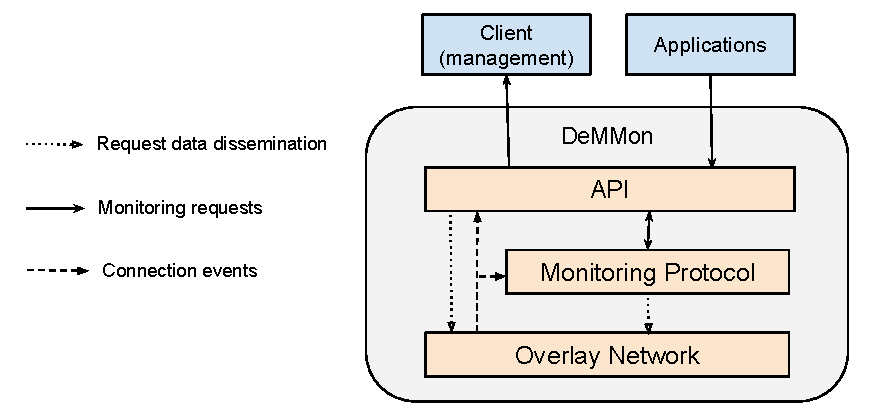
\includegraphics[width=\textwidth]{Chapters/Figures/DeMMon-arch-overview.pdf}
    \caption{An overview of the architecture of DeMMon}
    \label{fig:demmon-overview}
\end{figure}


\begin{enumerate}
    \item The overlay network, which strives to build the tree-shaped network, nodes in this network use proximity and a set of logical rules to change their location in the tree.

    \item The monitoring protocol, which is a component that collects and disseminates information using the overlay network's established connections. It communicates via notifications and asynchronous request-replies with the overlay network to receive updates regarding established connections and connection failures. Lastly, it receives requests from the API to collect information.

    \item Lastly, the API receives updates from both the overlay network and the monitoring protocol, exposes the received information from those layers, and allows ingestion of new information. Furthermore, it allows issuing commands to collect new information, perform local aggregations periodically, or trigger issued alarms based on the respective conditions.
\end{enumerate}

\section{Overlay network}

In this section, we discuss the design of the overlay network, which aims to build and maintain a latency and bandwidth aware tree-shaped network. We begin by providing the considered system model, then follow with an overview of the mechanisms responsible for building and maintaining the tree. Lastly, we conclude the chapter with a summary and discussion of the protocol.

\subsection{System Model}

The system model is assumed to be an asynchronous distributed scenario composed of nodes connected to the internet set-up such that they can send and receive messages via the internet (i.e. with an external IP or port-forwarding). We also assume that nodes are in both cloud and edge environments, with nodes possibly spread throughout multiple continents and with varied bandwidth values. All nodes run the same software stack with similar configuration settings, installed a priori.

Regarding the fault model, we assume that nodes fail in a crash-fault manner, stopping the emission and reception of all messages. Furthermore, in this system model all but a small portion of nodes (also known as the landmarks) can fail, as these are representative of nodes in data-centers, and consequently have increased fault-tolerance when compared to nodes in edge environments.

\subsection{Overview}

The devised membership protocol is coalesced by four main mechanisms: (1) the \textbf{join} mechanism, which aims to establish the initial tree structure (i.e. the parents and siblings of a node), (2) the \textbf{active view maintenance}, responsible for periodically sharing some information with the parent, and using that information for optimizations, (3) \textbf{passive view maintenance}, responsible for collecting information about peers which are not in the active view, used for fault tolerance and for optimizing the tree, and finally, (4) \textbf{fault tolerance}.

\subsubsection{Join mechanism}

As previously mentioned, the join mechanism is the mechanism responsible for creating the initial tree structure. This is executed by each node entering the system, and aims to establish an initial parent for the joining node.

\ref{alg:join:state}

% JOIN -----

% Types :

% Node {
%     ID \Comment{ string attributed by parent \asdupon[entering the syst]m}
%     measuredLatency \Comment{ the measured latency to the peer}
%     parentIP \Comment{ the IP of the parent of the Node}
%     nrChildren \Comment{ the number of children}
%     replied \Comment{ wether the node replied to joinMessage}
%     IP \Comment{ the node IP}
%     children: [] {
%         ID  \Comment{ the children id of the peer}
%         nrChildren  \Comment{ the nr of children of the child}
%         IP \Comment{ the node IP}
%     }
% }

\begin{algorithm}
% \setstretch{0.85}
\begin{algorithmic}[1]
    \caption{Join Protocol (part 1)}
    \asdtypes
        \State Node \{
        \Indent
            \State ID \Comment{ string attributed by parent upon entering the system}
            \State measuredLatency \Comment{ the measured latency to the peer}
            \State parentIP \Comment{ the IP of the parent of the Node}
            \State nrChildren \Comment{ the number of children}
            \State replied \Comment{ wether the node replied to joinMessage}
            \State IP \Comment{ the node IP}
            \State bw \Comment{the node's bandwidth}
            \State coordinates \Comment{ the node's coordinates}
            \State children: []Node \Comment{ the node's children, can be null for certain nodes (i.e. siblings and node's children), and is not sent in messages }
        \EndIndent
    \asdend
    \asdstate
        \State minGroupSize \Comment{ number representing the minimum group size}
        \State joinTimeouts \Comment{ collection of contacted nodes -> timerIDs}
        \State contactedNodes \Comment{ collection of all successfully contacted nodes}
        \State nodesToContact \Comment{ nodes being contacted}
        \State bestPeerLastLevel : Node \Comment{ lowest latency node in last level}
        \State landmakrs : []Node \Comment{ the ips of landmarks}
        \State isLandmark \Comment{ boolean indicating if self is landmark}
        \State joinTimeoutTimerID \Comment{ timerID for join messages}
        \State self : Node \Comment{ myself}
        \State siblings : Node \Comment{ my siblings}
        \State children : \{\} Node \Comment{ my children}
        \State parent : \{\} Node \Comment{ my parent}
    \asdend

\end{algorithmic}
\end{algorithm}

\begin{algorithm}
% \setstretch{0.85}
\begin{algorithmic}[1]

\caption{Join Protocol (part 2)}
\asdupon[Init(landmarks : map{IP}:Node, selfIP)]
        \State joinTimeouts \asdassign \{\}
        \State bestPeerLastLevel \asdassign \{\}
        \State landmarks \asdassign []
        \State isLandmark \asdassign selfIP \asdin landmarks
        \If{isLandmark}
            \State self \asdassign landmarks[selfIP]
            \For{landmark in landmarks}
                \State siblings \asdassign siblings + landmark
                \State redialUntilSuccess(landmark)
                \State measureUntilSuccess(landmark)
            \EndFor
        \Else 
            \State progressToNextLevel(landmarkIps)
        \EndIf
    \asdend
    
\asdupon[JoinTimeoutTimer(L)]
        \If{(L in Landmarks)}
            \State rejoinLater()
        \Else
            \State delete(nodesToContact[L])
        \EndIf
    \asdend
    
\asdupon[receive(Join<>,sender)]
        \State cancelTimer(joinTimeouts[sender])
        \State delete(joinTimeouts, sender)
        \State sendMessageSideChannel(JoinReply<self.parent, self.node, self.children>, sender)
    \asdend
    
\asdupon[receive JoinReply(<parentIP, node, children>, sender)]
        \State contactedNode \asdassign nodesToContact[node.IP]
        \State contactedNode.id \asdassign node.ID
        \State contactedNode.parentIP \asdassign parentIP
        \State contactedNode.nrChildren \asdassign len(children)
        \State contactedNode.replied \asdassign true
        \State contactedNode.children \asdassign children
    \asdend
   
\asdupon[NodeMeasured(node, latency)]
        \If{node $\in$ landmarkIPs}
            \State self.coordinates[landmarkIPs.indexOf(node)] = measuredLatency
        \EndIf
        \State nodesToContact[node].measuredLatency = latency
        \State nodesToContact[node].measured = true
    \asdend
        
\asdupon[NodeMeasuringFailed(node)]
    \State delete(nodesToContact, node)
\asdend

\asdprocedure[progressToNextLevel(nodeIPs)]
    \State nodesToContact \asdassign \{\}
    \State parentID \asdassign  nil
    \If{bestPeerLastLevel != nil}
        \State parentID \asdassign  bestPeerLastLevel.ID
    \EndIf
    \For{p in nodeIPs}
        \State nodesToContact[p] = Node \{IP: p, replied:false,measured: false\}
        \State MeasureNodeOnce(p) 
        \State sendMessageSideChannel(JoinMessage<>, p)
        \State t \asdassign setupTimer(JoinTimeoutTimer(p))
        \State joinTimeouts[p] = t
    \EndFor
\asdend

\end{algorithmic}
\end{algorithm}

\begin{algorithm}
% \setstretch{0.85}
\begin{algorithmic}[1]
\caption{Join Protocol (part 3)}
    
\asdupon[(forall n $\in$ nodesToContact -> n.measured \&\& n.replied)]
        \If{ len(nodesToContact) == 0}
            \If{bestPeerLastLevel == nil} \Comment{has not gotten past landmarks}
                \State rejToinLater()
                \State return
            \EndIf
        \EndIf
        \State contactedNodes.appendAll(nodesToContact)
        \For{node in sortedByLatency(nodesToContact)}
            \If{bestPeerLastLevel != nil}
                \If{bestPeerLastLevel.measuredLatency $\le$ node.measuredLatency} 
                    \State joinAsChild(bestPeerLastLevel)
                    \State return
                \EndIf
            \EndIf
            \If{(\asdnotin{node.IP}{landmarks}) \&\& node.nrChildren == 0}
                \State continue \Comment{ check if node has enough children to become joiner's parent (unless its a landmark)}
            \EndIf
            \State bestPeerLastLevel = node
            \State progressToNextLevel([c.IP for c in node.children])
            \State return
            \If{bestPeerLastLevel.parentIP == nil}
                \State bestPeerLastLevel = contactedNodes[bestPeerLastLevel.parentIP]
                \State joinAsChild(bestPeerLastLevel)       
                \State return
            \Else
                \State rejoinLater()
                \State return
            \EndIf
        \EndFor
    \asdend
   
    \asdprocedure[joinAsChild(p)]
        \State joinTimeoutTimerID = setupTimer(JoinRequestTimeout<p>)
        \State sendMessageSideChannel(JoinRequest<>, p.IP)
    \asdend

    \asdupon[JoinRequestTimeout(p)]
        \If{p.parentIP != nil}
            \State bestPeerLastLevel = contactedNodes[bestPeerLastLevel.parentIP]
            \State joinAsChild(bestPeerLastLevel)
        \Else
            \State rejoinLater()
        \EndIf
    \asdend

    \asdupon[receive(JoinRequest<>, sender)]
        \State generatedID \asdassign addChildren(sender) \Comment{ measures node and sets up periodic exchanges of information }

        \State sendMessageSideChannel(JoinRequestReply<generatedID,self,children>, p.IP)
    \asdend
        
    \asdupon[receive(JoinRequestReply<attributedId,parent,siblings>, sender)]
        \State addParent(sender) \Comment{ measures node and sets up periodic exchanges of information}
        \State addSiblings(siblings) \Comment{ measures nodes and sets up connections}
        \State self.id = parent.ID + "/" + attributedId
        \State cancelTimer(joinTimeoutTimerID)
    \asdend
\end{algorithmic}
\end{algorithm}


\subsubsection{Active view optimization}

\begin{algorithm}
    % \setstretch{0.85}
    \begin{algorithmic}[1]

        \caption{Membership protocol (Active view Optimization)}

        \asdstate
        \State childrenLatencies : dict<string:dict<string:number>>
        \asdend

        \asdrepeateveryx{config.updateChildPeriodicity}
        \If{parent != nil}
        \State sLatencies = set()
        \For{sibling in siblings}
        \State sLatencies.append(<sibling.IP,sibling.measuredLatency)
        \EndFor
        \State sendMessage(UpdateChildStatus<children, siblingLatencies>, parent)
        \EndIf
        \asdend

        \asdrepeateveryx{config.updateParentPeriodicity}
        \For{child in chidren}
        \State sendMessage(UpdateParentStatus<self,child.ID, parent>)
        \EndFor
        \asdend

        \asdupon[receive(UpdateParentStatus<parent,myID, grandParent>, sender)]
        \If{sender == parent.IP}
        \State parent = parent
        \State self.ID = parent.ID + myID
        \State grandParent = grandParent
        \EndIf
        \asdend

        \asdupon[receive(UpdateChildStatus<child, childSiblingLatencies>, sender)]
        \If{children[sender] != nil}
        \State children[sender] = children
        \State childrenLatencies[sender]=childSiblingLatencies
        \EndIf
        \asdend

        \asdrepeateveryx{config.updateChildPeriodicity}
        \State childrenLatValues = set()
        \For{c1 in children}
        \For{<c2, lat> in childrenLatencies[c]}
        \If{lat - c1.measuredLatency >= d.config.maxLatDowngrade}
        \State break
        \EndIf
        \State higherBwC = c1
        \State lowerBWC = c2
        \If{c2.bw > c1.bw}
        \State higherBwC = c2
        \State lowerBWC = c1
        \EndIf
        \State childrenLatValues.add(<higherBwC,lowerBWC,lat>)
        \EndFor
        \EndFor
        \State kickedNodes = set()
        \State newParents = set()
        \State potentialChildren = dict<string,set<Node>>
        \State sortByLatency(childrenLatValues)

        \For{<higherBwC,lowerBWC,lat> in childrenLatValues}
        \If{len(children) - len(kickedNodes) <= config.MinGroupSize}
        \State break
        \EndIf
        \If{higherBwC in kickedNodes or lowerBWC in kickedNodes}
        \State continue
        \EndIf
        \If{loserBWC in newParents}
        \State continue
        \EndIf
        \If{higherBwNode.nrChildren == 0}
        \State potentialChildren[higherBwNode].append(lowerBWC)
        \If{len(potentialChildren) >= config.MinGroupSize}
        \For{potentialChild in potentialChildren[higherBwNode]}
        \State newParents <- newParents + higherBwNode
        \State send(OptimizationPropose<higherBwNode>, potentialChild)
        \State higherBwNode.nrChildren++
        \State kickedNodes <- kickedNodes + potentialChild
        \EndFor
        \For{<nIP,potentialChilren> in potentialChildren}
        \State potentialChilren.deleteAll(potentialChildren[higherBwNode])
        \EndFor
        \State potentialChildren[higherBwNode] = set<Node>
        \State continue
        \EndIf
        \EndIf
        \State kickedNodes <- kickedNodes + lowerBWC
        \State send(OptimizationPropose<higherBwNode>, lowerBWNode)
        \EndFor
        \asdend

        \asdupon[receive(OptimizationPropose<newParent>, sender)]
        \If{sender == parent}
        \State send(OptimizationProposeRequest<sender>, newParent)
        \EndIf
        \asdend

        \asdupon[receive(OptimizationProposeRequest<p>, sender)]
        \If{ p == parent \&\& sender in siblings} \Comment{ parent issuing the message is the same parent that i have}
        \State send(OptimizationProposeRequestReply<true>, sender)
        \Else
        \State sendSideChannel(OptimizationProposeRequestReply<false>, sender)
        \EndIf
        \asdend

        \asdupon[receive(OptimizationProposeRequestReply<reply>, sender)]
        \If{reply}
        \State sendMessageAndDisconnectFrom(DisconnectMessage<>, parent)
        \State addParent(sender)
        \EndIf
        \asdend

    \end{algorithmic}
\end{algorithm}

\subsubsection{Passive view optimization}

\begin{algorithm}
\begin{algorithmic}[1]

        \caption{Oportunistic Optimization}

    \asdstate
        \State childrenLatencies : dict<string:dict<string:number>>
    \asdend

    \asdrepeateveryx[config.OportunisticOptimizationTimeout]
        \State toMeasureRand = getRandSample(eView, config.NrPeersToMeasureRandom)
        \State toMeasureBiasedOpts = sortByEuclideanDist(eView / toMeasureRand)
        \State toMeasureBiased = getRandSample(toMeasureBiasedOpts, config.NrPeersToMeasureRandom)

        \For p in toMeasureRand:
            \State measurePeer(p)
        \EndFor
        \For p in toMeasureBiased:
            \State measurePeer(p)
        \EndFor
    \asdend

    \asdupon{peerMeasured(p, latency)}
        \State latencyImprovement := parent.measuredLatency - Latency
        \If{latencyImprovement >= config.MinLatencyForImprovement}:
            \State sendMessageSideChannel(OportunisticImprovementReq<self>,p)
        \EndIf
    \asdend


    \asdupon{receive(OportunisticImprovementReq<p>,sender)}
        \If{isDescendent(p.ID,self)}:
            \State sendMessageSideChannel(OportunisticImprovementReqReply<false>,sender)
        \Else
            \State addChildren(sender)
            \State sendMessageSideChannel(OportunisticImprovementReqReply<true>,sender)
        \EndIf
    \asdend

    \asdupon{receive(OportunisticImprovementReqReply<answer>,sender)}
        \If {answer} 
            \State addParent(sender)
        \EndIf
    \asdend

\end{algorithmic}
\end{algorithm}

\subsubsection{Fault tolerance}

\subsection{Summary}

\section{Monitoring protocol}

\subsection{Overview}

\subsection{Aggregation mechanisms}

\subsubsection{Single root aggregation}

\subsubsection{Multi root aggregation}

\subsubsection{Neighborhood aggregation}

\subsection{Summary}

\section{API}

\subsection{System Model}

\subsection{Overview}

\subsection{Showcase}
